\section{Investigation}

\todo{Introducory paragraph about how we're focussing on the single core case}

Current state-of-the-art processors are based on Complimentary Metal Oxide Semiconductor (CMOS) technology and multi- and many-core super-scalar architectures. The limits of these technologies are fast  approaching, however, and research into the next generation of power-efficient architectures and semiconductor fabrication techniques is under way \cite{esmaeilzadeh:2011aa}.

The power draw of CMOS chips can be divided into the components as described by \autoref{eq:totpwr}, the most significant of which are dynamic and leakage power. Dynamic power refers to power consumed as logic gates change state while a processor performs work. Leakage power stems from the fact that at very small scales the insulating properties of silicon break down, allowing some current to leak out even when gates remain inactive. Other forms of power dissipation exist, however their effects are relatively minor \cite{kaxiras:2008aa}.


\begin{equation}
\label{eq:totpwr}
P_{tot} = P_{dyn} + P_{leak} + P_{other}
\end{equation}
\begin{equation} 
\label{eq:dynpwr}
P_{dyn} \propto CV^{2}Af
\end{equation}

\autoref{eq:dynpwr} is a common approximation for dynamic power in which C denotes load capacitance, $V$ the supply voltage, $A$ the activity factor and $f$ the clock frequency. Of these, only activity factor is directly related to processor workload as it captures the percentage of logic elements which change state each clock cycle. Conversely, capacitance is a fixed value arising from the wire lengths of on-chip structures.

Processor frequency and supply voltage may also be influenced by workload through the actions of Dynamic Voltage and Frequency Scaling (DVFS) activity. These properties vary in tandem, taking on predetermined values dependent on a hardware-specific number of fixed P-States. To paraphrase, DVFS can act to reduce the clock speed of underutilized processors. When this happens, voltage requirements also decrease.

Unsurprisingly, leakage power is less sensitive to processor workload as it as it does not 
\todo{mention that leakage is linear in terms of frequency, whereas dynamic power is effectively cubic in terms of frequency and linear in terms of activity factor.}


\todo{On the nature of software power optimizations... }
We can either reduce activity factor directly or work to tune software to be more dvfs friendly.\todo{Intel energy efficiency optimization guide citation...}

\todo{Different processor subsystems operate at different frequencies. The clock distribution network operates at $\alpha=1$.}
\todo{Clock gating, in which processor elements are isolated from the clock signal and cease to function. When this happens, their activity factor, and hence dynamic power consumption, is zero.}



\todo{REWORD:
As previously mentioned, only dynamic power consumption may be reduced through code optimizations. \autoref{eq:dynpwr} shows that if an optimization leads to a reduction in activity factor then there will be a corresponding reduction in power consumption. 
Activity factor and CPU occupancy are the two factors which should be reduced in order to realize power optimization. 
}


An important feature of the equations governing power draw is that only $P_{dyn}$ is directly influenced by software, in particular due to its inclusion of the $A$ term. Software can also indirectly effect both dynamic and leakage current if it triggers changes to clock frequency and therefore supply voltage through DVFS. \todo{Ensure define dvfs} \todo{reword this bit - no equations now}

Historically, dynamic power has been the biggest contributor to $P_{tot}$, however leakage power has been on track to overtake it since the breakdown of Dennard Scaling.  Sub-threshold and gate-oxide leakage dominate total leakage current, and they both increase exponentially as transistors shrink. Process improvements like the introduction of high-k dielectric materials~\cite{jan:2009aa} have kept leakage power in check over the last decade, however there is no avoiding the fact that insulating properties will degrade as transistors get smaller.

\begin{figure}
\centering
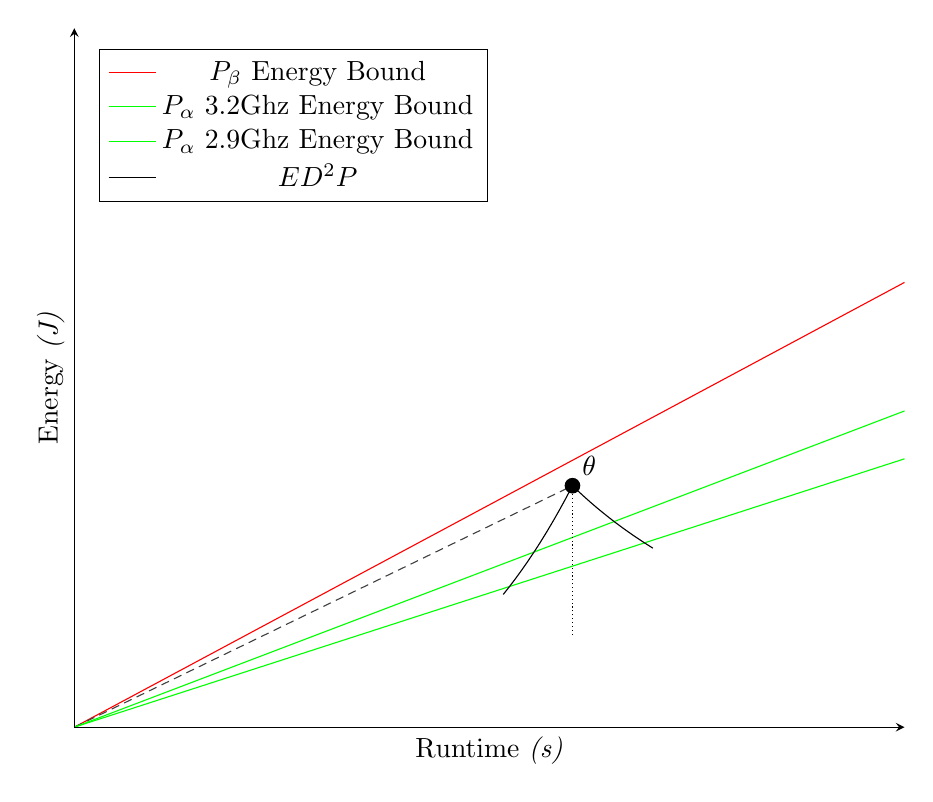
\begin{tikzpicture}
  \begin{axis}[ticks = none, 
    axis on top,
    axis x line=bottom,
    axis y line=left,
  	xlabel={Runtime \emph{(s)}},
    ylabel={Energy \emph{(J)}},    
    xmin=0, xmax=50,
    ymin=0, ymax=3300,
    width=\linewidth,
    legend style={legend pos=north west}
    ]

    %% Model Parameters %%

    \pgfmathsetmacro{\baselinepower}{14.56} % NOP code
    \pgfmathsetmacro{\rooflinepower}{42.00}
    \pgfmathsetmacro{\codepower}{38} 
    \pgfmathsetmacro{\codetime}{30}

    %% Intermezzo Values %%
    \pgfmathsetmacro{\codeenergy}{\codepower * \codetime}
    \pgfmathsetmacro{\baselineenergy}{\baselinepower * \codetime}
    \pgfmathsetmacro{\rooflineenergy}{\rooflinepower * \codetime}
    \pgfmathsetmacro{\lowdisplayline}{(2 * \baselinepower + \codepower) / 3}
    \pgfmathsetmacro{\highdisplayline}{(1 * \rooflinepower + 1 * \codepower) / 2}

    % arguments: code power, code time, x, n 
    \pgfmathdeclarefunction{metricbound}{4}{%
      \pgfmathparse{((#1 * #2^(#4 + 1)) / #3^#4)}%
    }
    \pgfmathdeclarefunction{definitionbound}{4}{%
      \pgfmathparse{((#1 / #2^(#4 + 1)) * #3^(#4 + 2))}%
    }
 
    % BETA ROOFLINE BOUND
    \addplot[color=red, domain=\pgfkeysvalueof{/pgfplots/xmin}:\pgfkeysvalueof{/pgfplots/xmax}] {\rooflinepower * x};
    \addlegendentry{$P_{\beta}$ Energy Bound}

    %const power diagonal
    \addplot[color=darkgray, densely dashed, forget plot, %forget plot prevents legend entry
            domain=\pgfkeysvalueof{/pgfplots/xmin}:\codetime] {\codepower * x}; 

    % ALPHA BASELINE BOUND 3.2 
    \addplot[color=green, domain=\pgfkeysvalueof{/pgfplots/xmin}:\pgfkeysvalueof{/pgfplots/xmax}] {29.86 * x};
    \addlegendentry{$P_{\alpha}$ 3.2Ghz Energy Bound} 


    % ALPHA BASELINE BOUND 2.9
    \addplot[color=green, domain=\pgfkeysvalueof{/pgfplots/xmin}:\pgfkeysvalueof{/pgfplots/xmax}] {25.34 * x};
    \addlegendentry{$P_{\alpha}$ 2.9Ghz Energy Bound} 



    % Constant Time vertical dots
    %vertical
    \draw[densely dotted] ({axis cs:\codetime,\baselineenergy}) -- ({axis cs:\codetime,\codeenergy});

    % Sadly, pgfplots sucks too much to calculate cube roots
    % Domain values are calculated with a ruby script in tools

    %% Energy Delay Squared Product Area ##
    \addplot[domain=25.83028:34.84283] { min(definitionbound(\codepower, \codetime, x, 2),metricbound(\codepower, \codetime, x, 2))};
    \addlegendentry{$ED^2P$}




     \node[circle,fill,inner sep=2pt] at (axis cs:\codetime,\codeenergy) {};
    \node[above right] at (axis cs:\codetime,\codeenergy) {$\theta$};
  \end{axis}
\end{tikzpicture}

\caption{Multiple Baseline CODENAME Optimization Space}
\label{fig:multibaseline-investigation}
\end{figure}

\begin{table}
\centering
\input{tab/tex/power_of_cores_x_freq.tex}
\caption{Base CPU Power (W)}
\end{table} 

\begin{table}
\centering
\input{tab/tex/code_metrics}
\caption{Rodinia Results, 4 cores at 3.2 GHz}
\end{table} 


\begin{figure}
\centering
\@ifundefined{pstateminimdtable}{%
  \pgfplotstableread[col sep=comma]{plot/minimd-pstates/data/pstate_power_4_cores.csv}\pstateminimdtable
}{}

\begin{tikzpicture}
  \begin{axis}[
    width=0.95\linewidth,
    axis on top,
    axis x line=bottom,
    axis y line=left,
  	xlabel={Runtime \emph{(s)}},
    ylabel={Energy \emph{(J)}},    
    xmin=0, xmax=60,
    ymin=0, ymax=1500,
    legend columns=2,
    legend to name=minimd-pstate:legend,
    legend style={/tikz/every even column/.append style={column sep=0.2cm}} % space out columns a bit
    ]

    %% Model Parameters %%
    \pgfplotstablegetelem{0}{Runtime}\of{\pstateminimdtable}
    \pgfmathsetmacro{\codetime}{\pgfplotsretval} 
    \pgfplotstablegetelem{0}{Energy}\of{\pstateminimdtable}
    \pgfmathsetmacro{\codeenergy}{\pgfplotsretval} 
    \pgfmathsetmacro{\baselinepower}{13.510238}

    %% Intermezzo Values %%
    \pgfmathsetmacro{\codepower}{\codeenergy / \codetime}

    % arguments: code power, code time, x, n 
    \pgfmathdeclarefunction{metricbound}{4}{%
      \pgfmathparse{((#1 * #2^(#4 + 1)) / #3^#4)}%
    }
    \pgfmathdeclarefunction{definitionbound}{4}{%
      \pgfmathparse{((#1 / #2^(#4 + 1)) * #3^(#4 + 2))}%
    }

    % ALPHA BASELINE BOUND 
    \addplot[color=printgreen, very thick, name path=basebound, domain=\pgfkeysvalueof{/pgfplots/xmin}:\pgfkeysvalueof{/pgfplots/xmax}] {\baselinepower * x};
    \addlegendentry{$P_{min}$ Energy Bound} 


    %% 3.2 GHz start point
    \pgfmathsetmacro{\blnodex}{23.77199310523716}
    \pgfmathsetmacro{\brnodex}{38.6049404590049}
    \addplot[name path=edpdef, draw=none, domain=\blnodex:\codetime+1, forget plot] {definitionbound(\codepower, \codetime, x, 2)};
    \addplot[name path=edpopt, draw=none, domain=\codetime-1:\brnodex, forget plot] {metricbound(\codepower, \codetime, x, 2)};

    \path[name path=edpspace,
      intersection segments={
        of=edpdef and edpopt,
        sequence=A0 -- B1,
      }
      ]; 
    \addplot[blue!20] fill between[of=edpspace and basebound]; 
    \addlegendentry{3.2 GHz POSE}

    %% PState progression
    \addplot[mark=x, black] table[x=Runtime,y=Energy, trim cells=true] {\pstateminimdtable}
      node[pos=0.0, pin=left:3.2 GHz]{}
      node[pos=1.0, pin=95:1.6 GHz]{}
      node[pos=0.5745, pin={[pin distance=0.15cm] above:2.2 GHz}]{}
    ;
    \addlegendentry{P-state Progression}

    %%
    \pgfmathsetmacro{\codetime}{31.160996}
    \pgfmathsetmacro{\codepower}{26.555410070974624}
    \pgfmathsetmacro{\blnodex}{24.876044579784466}
    \addplot[name path=edpdef, gray, densely dashed, domain=\blnodex:\codetime, forget plot] {definitionbound(\codepower, \codetime, x, 2)};

    %%
    \pgfmathsetmacro{\codetime}{32.221644}
    \pgfmathsetmacro{\codepower}{25.19066851461707}
    \pgfmathsetmacro{\blnodex}{26.17914532437151}
    \addplot[name path=edpdef, gray, densely dashed, domain=\blnodex:\codetime, forget plot] {definitionbound(\codepower, \codetime, x, 2)};

    %%
    \pgfmathsetmacro{\codetime}{33.189564}
    \pgfmathsetmacro{\codepower}{24.052689996168674}
    \pgfmathsetmacro{\blnodex}{27.384280155637242}
    \addplot[name path=edpdef, gray, densely dashed, domain=\blnodex:\codetime, forget plot] {definitionbound(\codepower, \codetime, x, 2)};

    %%
    \pgfmathsetmacro{\codetime}{35.548669}
    \pgfmathsetmacro{\codepower}{21.708309894809283}
    \pgfmathsetmacro{\blnodex}{30.35072062021389}
    \addplot[name path=edpdef, gray, densely dashed, domain=\blnodex:\codetime, forget plot] {definitionbound(\codepower, \codetime, x, 2)};

    %%
    \pgfmathsetmacro{\codetime}{36.852917}
    \pgfmathsetmacro{\codepower}{20.791885293639034}
    \pgfmathsetmacro{\blnodex}{31.919904165043228}
    \addplot[name path=edpdef, gray, densely dashed, domain=\blnodex:\codetime, forget plot] {definitionbound(\codepower, \codetime, x, 2)};

    %%
    \pgfmathsetmacro{\codetime}{38.225746}
    \pgfmathsetmacro{\codepower}{19.926273930664426}
    \pgfmathsetmacro{\blnodex}{33.58161699951163}
    \addplot[name path=edpdef, gray, densely dashed, domain=\blnodex:\codetime, forget plot] {definitionbound(\codepower, \codetime, x, 2)};

    %%
    \pgfmathsetmacro{\codetime}{39.720356}
    \pgfmathsetmacro{\codepower}{19.032817706870503}
    \pgfmathsetmacro{\blnodex}{35.432334683311204}
    \addplot[name path=edpdef, gray, densely dashed, domain=\blnodex:\codetime, forget plot] {definitionbound(\codepower, \codetime, x, 2)};

    %%
    \pgfmathsetmacro{\codetime}{41.430395}
    \pgfmathsetmacro{\codepower}{18.26008617586195}
    \pgfmathsetmacro{\blnodex}{37.47190734697387}
    \addplot[name path=edpdef, gray, densely dashed, domain=\blnodex:\codetime, forget plot] {definitionbound(\codepower, \codetime, x, 2)};

    %% 2.2GHz
    \pgfmathsetmacro{\codetime}{43.161913}
    \pgfmathsetmacro{\codepower}{17.552650110758528}
    \pgfmathsetmacro{\blnodex}{39.55555231782452}
    \addplot[name path=edpdef, red, densely dashed, domain=\blnodex:\codetime] {definitionbound(\codepower, \codetime, x, 2)};
    \addlegendentry{Optimisation Cutoff}

    %%
    \pgfmathsetmacro{\codetime}{45.85507}
    \pgfmathsetmacro{\codepower}{16.61222678321067}
    \pgfmathsetmacro{\blnodex}{42.802165661611}
    \addplot[name path=edpdef, gray, densely dashed, domain=\blnodex:\codetime, forget plot] {definitionbound(\codepower, \codetime, x, 2)};

    %%
    \pgfmathsetmacro{\codetime}{49.7305}
    \pgfmathsetmacro{\codepower}{15.67846259337831}
    \pgfmathsetmacro{\blnodex}{47.323406701270244}
    \addplot[name path=edpdef, gray, densely dashed, domain=\blnodex:\codetime, forget plot] {definitionbound(\codepower, \codetime, x, 2)};

    %%
    \pgfmathsetmacro{\codetime}{52.358683}
    \pgfmathsetmacro{\codepower}{15.137478343372388}
    \pgfmathsetmacro{\blnodex}{50.41098720057872}
    \addplot[name path=edpdef, gray, densely dashed, domain=\blnodex:\codetime, forget plot] {definitionbound(\codepower, \codetime, x, 2)};

    %%
    \pgfmathsetmacro{\codetime}{55.340763}
    \pgfmathsetmacro{\codepower}{14.650088958838532}
    \pgfmathsetmacro{\blnodex}{53.866578212248804}
    \addplot[name path=edpdef, gray, densely dashed, domain=\blnodex:\codetime, forget plot] {definitionbound(\codepower, \codetime, x, 2)};

    %%
    \pgfmathsetmacro{\codetime}{58.637567}
    \pgfmathsetmacro{\codepower}{14.09304050763225}
    \pgfmathsetmacro{\blnodex}{57.81786383949271}
    \addplot[name path=edpdef, gray, densely dashed, domain=\blnodex:\codetime, forget plot] {definitionbound(\codepower, \codetime, x, 2)};


 \end{axis}
\end{tikzpicture}

\caption{MiniMD Pstate Optimization Space}
\label{fig:minimd-pstates}
\end{figure}



